\chapter{Development and Simulation}\label{ch:ch2label}
\section{Arduino IDE}
The code to be burnt to the program memory of an \arduino{} is written and compiled in the \emph{Arduino IDE}. The IDE also has a serial monitor, which displays values being recieved in real-time from the Arduino via serial communication through the serial port (COM ports). The IDE verifies for correct C/C++ syntax and compiles it, before linking it to Arduino Library files. This creates the \textit{hex} file that contains the code in binary form. It can either be uploaded to the board directly, which the IDE does with the help of the Bootloader program pre-installed on the Arduino, or it can be fed to a \emph{simulator}, which would simulate and show how the circuit would run and its associated parameters.
\begin{figure}[H]
	\vfill
	\centering
	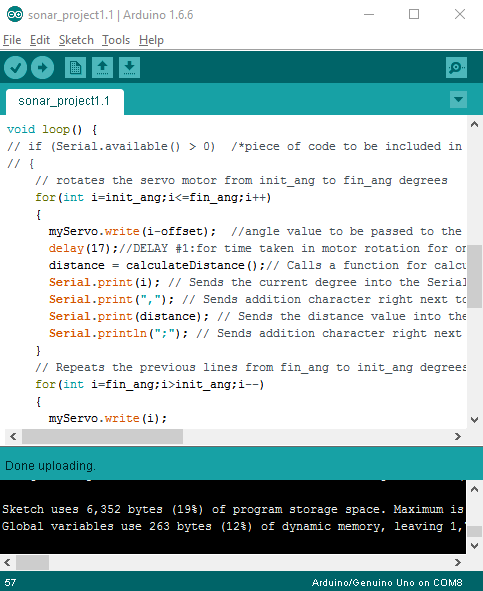
\includegraphics[width=0.5\textwidth]{../Files/IDE}
	\caption{The Arduino IDE}  \label{fig:IDE}
\end{figure}

%\cite{Madsen2010}, \cite{Oetiker2010} and \cite{Mittelbach2005}.

\clearpage
